%---------------- Financial Plan ----------------%
\section{Financial Plan}

\subsection{Financial Requirements}

\textbf{Startup Capital Requirements:}

\begin{tabular}{|l|r|}
\hline
\textbf{Item} & \textbf{Amount (UGX)} \\
\hline
Equipment and furniture & 8,500,000 \\
Initial inventory (products) & 1,500,000 \\
Facility renovation and setup & 2,500,000 \\
Signage and branding & 400,000 \\
Business registration and licenses & 300,000 \\
Initial marketing campaign & 500,000 \\
Working capital (3 months) & 3,000,000 \\
Contingency fund (10\%) & 1,670,000 \\
\hline
\textbf{Total Startup Capital} & \textbf{18,370,000} \\
\hline
\end{tabular}

\vspace{1em}

% Startup Capital Breakdown Chart
\begin{center}
\textbf{Startup Capital Allocation}
\vspace{0.5em}

\begin{tikzpicture}
    \pie[
        text=legend,
        radius=2.8,
        color={primarycolor!70, secondarycolor!70, accentcolor!70, 
               primarycolor!40, secondarycolor!40, accentcolor!40, 
               lightgray, primarycolor!20}
    ]{
        46/Equipment \& Furniture (8.5M),
        14/Facility Renovation (2.5M),
        16/Working Capital (3M),
        9/Contingency (1.67M),
        8/Initial Inventory (1.5M),
        3/Marketing (0.5M),
        2/Signage (0.4M),
        2/Registration (0.3M)
    }
\end{tikzpicture}
\end{center}

\vspace{1em}

\textbf{Monthly Operating Expenses:}

\begin{tabular}{|l|r|}
\hline
\textbf{Expense Category} & \textbf{Amount (UGX)} \\
\hline
Rent & 500,000 \\
Staff salaries & 1,300,000 \\
Products and supplies & 400,000 \\
Utilities (water, electricity) & 180,000 \\
Internet and phone & 100,000 \\
Marketing & 150,000 \\
Maintenance and repairs & 80,000 \\
Insurance & 50,000 \\
Miscellaneous & 100,000 \\
\hline
\textbf{Total Monthly Expenses} & \textbf{2,860,000} \\
\hline
\end{tabular}

\vspace{1em}

% Monthly Operating Expenses Chart
\begin{center}
\textbf{Monthly Operating Expenses Breakdown}
\vspace{0.5em}

\begin{tikzpicture}
    \begin{axis}[
        xbar,
        width=12cm,
        height=8cm,
        xlabel={Amount (Million UGX)},
        symbolic y coords={Miscellaneous, Insurance, Maintenance, Marketing, 
                          Internet, Utilities, Products, Rent, Salaries},
        ytick=data,
        nodes near coords,
        nodes near coords align={horizontal},
        xmin=0,
        xmax=1.5,
        bar width=15pt,
        enlarge y limits=0.1
    ]
    
    \addplot[fill=primarycolor!70] coordinates {
        (0.1, Miscellaneous)
        (0.05, Insurance)
        (0.08, Maintenance)
        (0.15, Marketing)
        (0.1, Internet)
        (0.18, Utilities)
        (0.4, Products)
        (0.5, Rent)
        (1.3, Salaries)
    };
    
    \end{axis}
\end{tikzpicture}

\vspace{0.5em}
Staff salaries represent the largest operating expense at 45\% of monthly costs.
\end{center}

\subsection{Financing Strategy}

\textbf{Funding Sources:}
\begin{itemize}[leftmargin=2em]
    \item \textbf{Personal Savings:} UGX 5,000,000 (27\%)
    \item \textbf{Family Contribution:} UGX 3,000,000 (16\%)
    \item \textbf{Bank Loan:} UGX 8,000,000 (44\%)
    \item \textbf{Youth/Student Grant:} UGX 2,370,000 (13\%)
    \item \textbf{Total:} UGX 18,370,000
\end{itemize}

\textbf{Loan Terms (if applicable):}
\begin{itemize}[leftmargin=2em]
    \item Loan amount: UGX 8,000,000
    \item Interest rate: 18\% per annum
    \item Repayment period: 3 years (36 months)
    \item Monthly payment: UGX 290,000 (approximately)
    \item Collateral: Business equipment and personal guarantee
\end{itemize}

\vspace{1em}

% Funding Sources Pie Chart
\begin{center}
\textbf{Funding Sources Distribution}
\vspace{0.5em}

\begin{tikzpicture}
    \pie[
        text=legend,
        radius=2.8,
        color={primarycolor!70, secondarycolor!70, accentcolor!70, lightgray}
    ]{
        44/Bank Loan (8M),
        27/Personal Savings (5M),
        16/Family Contribution (3M),
        13/Youth Grant (2.37M)
    }
\end{tikzpicture}
\end{center}

\vspace{1em}

% Loan Repayment Schedule
\begin{center}
\textbf{Loan Repayment Schedule (First 12 Months)}
\vspace{0.5em}

\begin{tikzpicture}
    \begin{axis}[
        ybar stacked,
        bar width=15pt,
        xlabel={Month},
        ylabel={Amount (UGX)},
        ymin=0,
        ymax=350000,
        xtick={1,2,3,4,5,6,7,8,9,10,11,12},
        width=14cm,
        height=7cm,
        legend pos=north east,
        grid=major,
        ymajorgrids=true
    ]
    
    % Principal payment
    \addplot[fill=primarycolor!70] coordinates {
        (1,170000) (2,172000) (3,174000) (4,176000) (5,178000) (6,180000)
        (7,182000) (8,184000) (9,186000) (10,188000) (11,190000) (12,192000)
    };
    
    % Interest payment
    \addplot[fill=secondarycolor!70] coordinates {
        (1,120000) (2,118000) (3,116000) (4,114000) (5,112000) (6,110000)
        (7,108000) (8,106000) (9,104000) (10,102000) (11,100000) (12,98000)
    };
    
    \legend{Principal, Interest}
    
    \end{axis}
\end{tikzpicture}

\vspace{0.5em}
Monthly loan payment of UGX 290,000 includes both principal and interest components.
\end{center}

\vspace{1em}

\begin{tcolorbox}[mybox, title=\textbf{Financing Strategy Rationale}]
\textbf{Why This Mix of Funding?}
\begin{itemize}[leftmargin=1em, itemsep=0pt]
    \item \textbf{Personal Savings (27\%):} Demonstrates commitment and reduces debt
    \item \textbf{Family Support (16\%):} Interest-free capital with flexible terms
    \item \textbf{Bank Loan (44\%):} Provides majority of capital while building credit history
    \item \textbf{Youth Grant (13\%):} Non-repayable funding reduces financial burden
\end{itemize}

\textbf{Debt Management Strategy:}
\begin{itemize}[leftmargin=1em, itemsep=0pt]
    \item Loan payments covered by projected profits from Month 4 onwards
    \item Maintain 3-month cash reserve for emergencies
    \item Option to make early repayments from excess profits
    \item Debt-to-equity ratio: 44\% (healthy level)
\end{itemize}
\end{tcolorbox}

\subsection{Financial Resources}

\textbf{Asset Base:}
\begin{itemize}[leftmargin=2em]
    \item Equipment and furniture: UGX 8,500,000
    \item Initial inventory: UGX 1,500,000
    \item Cash reserves: UGX 3,000,000
    \item Total assets at startup: UGX 13,000,000
\end{itemize}

\textbf{Financial Management:}
\begin{itemize}[leftmargin=2em]
    \item Separate business bank account
    \item Daily cash reconciliation
    \item Weekly financial review
    \item Monthly financial statements
    \item Quarterly financial analysis
    \item Annual audit
\end{itemize}

\textbf{Financial Controls:}
\begin{itemize}[leftmargin=2em]
    \item Dual authorization for large expenses (over UGX 500,000)
    \item Regular inventory audits
    \item Petty cash limit of UGX 100,000
    \item Monthly bank reconciliation
    \item Professional accounting software
    \item External accountant review quarterly
\end{itemize}

\subsection{Financial Projections}

\subsubsection{Income Statement (Year 1 Projection)}

\begin{tabular}{|l|r|r|r|}
\hline
\textbf{Item} & \textbf{Q1} & \textbf{Q2} & \textbf{Year 1} \\
\hline
\multicolumn{4}{|l|}{\textbf{Revenue}} \\
Service revenue & 22,500,000 & 42,000,000 & 180,000,000 \\
Product sales & 2,500,000 & 4,500,000 & 20,000,000 \\
\hline
\textbf{Total Revenue} & \textbf{25,000,000} & \textbf{46,500,000} & \textbf{200,000,000} \\
\hline
\multicolumn{4}{|l|}{\textbf{Cost of Goods Sold}} \\
Products and supplies & 3,600,000 & 6,000,000 & 28,000,000 \\
\hline
\textbf{Gross Profit} & \textbf{21,400,000} & \textbf{40,500,000} & \textbf{172,000,000} \\
\hline
\multicolumn{4}{|l|}{\textbf{Operating Expenses}} \\
Salaries and wages & 11,700,000 & 11,700,000 & 46,800,000 \\
Rent & 4,500,000 & 4,500,000 & 18,000,000 \\
Utilities & 1,620,000 & 1,620,000 & 6,480,000 \\
Marketing & 1,350,000 & 1,350,000 & 5,400,000 \\
Insurance & 450,000 & 450,000 & 1,800,000 \\
Maintenance & 720,000 & 720,000 & 2,880,000 \\
Miscellaneous & 900,000 & 900,000 & 3,600,000 \\
Depreciation & 425,000 & 425,000 & 1,700,000 \\
\hline
\textbf{Total Operating Expenses} & \textbf{21,665,000} & \textbf{21,665,000} & \textbf{86,660,000} \\
\hline
\textbf{Operating Profit} & \textbf{-265,000} & \textbf{18,835,000} & \textbf{85,340,000} \\
\hline
Interest expense & 360,000 & 360,000 & 1,440,000 \\
\hline
\textbf{Net Profit Before Tax} & \textbf{-625,000} & \textbf{18,475,000} & \textbf{83,900,000} \\
\hline
Tax (30\%) & 0 & 5,542,500 & 25,170,000 \\
\hline
\textbf{Net Profit After Tax} & \textbf{-625,000} & \textbf{12,932,500} & \textbf{58,730,000} \\
\hline
\end{tabular}

\vspace{1em}

\subsubsection{Income Statement (Year 1 Projection)}

\begin{tabular}{|l|r|r|r|r|}
\hline
\textbf{Item} & \textbf{Q1} & \textbf{Q2} & \textbf{Q3-Q4} & \textbf{Year 1} \\
\hline
\multicolumn{5}{|l|}{\textbf{Revenue}} \\
Service revenue & 4,800,000 & 9,800,000 & 21,600,000 & 36,200,000 \\
Product sales & 550,000 & 1,100,000 & 2,400,000 & 4,050,000 \\
\hline
\textbf{Total Revenue} & \textbf{5,350,000} & \textbf{10,900,000} & \textbf{24,000,000} & \textbf{40,250,000} \\
\hline
\multicolumn{5}{|l|}{\textbf{Cost of Goods Sold}} \\
Products and supplies & 970,000 & 1,960,000 & 4,320,000 & 7,250,000 \\
\hline
\textbf{Gross Profit} & \textbf{4,380,000} & \textbf{8,940,000} & \textbf{19,680,000} & \textbf{33,000,000} \\
\hline
\multicolumn{5}{|l|}{\textbf{Operating Expenses}} \\
Salaries and wages & 11,700,000 & 11,700,000 & 23,400,000 & 46,800,000 \\
Rent & 4,500,000 & 4,500,000 & 9,000,000 & 18,000,000 \\
Utilities & 1,620,000 & 1,620,000 & 3,240,000 & 6,480,000 \\
Marketing & 1,350,000 & 1,350,000 & 2,700,000 & 5,400,000 \\
Insurance & 450,000 & 450,000 & 900,000 & 1,800,000 \\
Maintenance & 720,000 & 720,000 & 1,440,000 & 2,880,000 \\
Miscellaneous & 900,000 & 900,000 & 1,800,000 & 3,600,000 \\
Depreciation & 425,000 & 425,000 & 850,000 & 1,700,000 \\
\hline
\textbf{Total Operating Expenses} & \textbf{21,665,000} & \textbf{21,665,000} & \textbf{43,330,000} & \textbf{86,660,000} \\
\hline
\textbf{Operating Profit} & \textbf{-17,285,000} & \textbf{-12,725,000} & \textbf{-23,650,000} & \textbf{-53,660,000} \\
\hline
Interest expense & 360,000 & 360,000 & 720,000 & 1,440,000 \\
\hline
\textbf{Net Profit Before Tax} & \textbf{-17,645,000} & \textbf{-13,085,000} & \textbf{-24,370,000} & \textbf{-55,100,000} \\
\hline
Tax (30\%) & 0 & 0 & 0 & 0 \\
\hline
\textbf{Net Profit After Tax} & \textbf{-17,645,000} & \textbf{-13,085,000} & \textbf{-24,370,000} & \textbf{-55,100,000} \\
\hline
\end{tabular}

\vspace{1em}

\textbf{Key Financial Metrics (Year 1):}
\begin{itemize}[leftmargin=2em]
    \item Gross profit margin: 82\%
    \item Operating loss: UGX 53.7M (investment phase)
    \item Revenue covers: 46\% of operating expenses
    \item Break-even requires: 15-18 customers/day (achievable in Year 2)
\end{itemize}

\vspace{1em}

\begin{tcolorbox}[mybox, title=\textbf{Understanding Year 1 Loss - This is Normal for Startups}]
\textbf{Why Year 1 Shows a Loss:}
\begin{itemize}[leftmargin=1em, itemsep=0pt]
    \item \textbf{Investment Phase:} Building foundation for future profitability
    \item \textbf{Fixed Costs:} Rent and salaries remain constant regardless of customer volume
    \item \textbf{Very Conservative Revenue:} Starting with only 3-5 customers/day
    \item \textbf{Normal for Service Businesses:} Most salons take 12-18 months to break even
    \item \textbf{Covered by Startup Capital:} Working capital budget includes this scenario
\end{itemize}

\textbf{Path to Profitability:}
\begin{itemize}[leftmargin=1em, itemsep=0pt]
    \item \textbf{Year 2:} UGX 70M revenue → UGX 15M profit (21\% margin)
    \item \textbf{Year 3:} UGX 105M revenue → UGX 28M profit (27\% margin)
    \item \textbf{Year 4:} UGX 145M revenue → UGX 42M profit (29\% margin)
    \item \textbf{Year 5:} UGX 190M revenue → UGX 55M profit (29\% margin)
    \item \textbf{Cumulative 5-year profit:} UGX 85M (excellent return despite Year 1 loss)
\end{itemize}

\textbf{Break-even Analysis:}
\begin{itemize}[leftmargin=1em, itemsep=0pt]
    \item Monthly fixed costs: UGX 2.86M
    \item Average revenue per customer: UGX 20,000
    \item Gross margin: 82\%
    \item Break-even customers/month: 174 (7 per day)
    \item Expected to reach break-even: Early Year 2 (Month 14-16)
\end{itemize}
\end{tcolorbox}

\vspace{1em}

% Revenue vs Expenses Chart
\begin{center}
\textbf{Year 1 Revenue vs Expenses (Quarterly)}
\vspace{0.5em}

\begin{tikzpicture}
    \begin{axis}[
        ybar,
        bar width=15pt,
        xlabel={Quarter},
        ylabel={Amount (Million UGX)},
        ymin=0,
        ymax=50,
        xtick=data,
        symbolic x coords={Q1, Q2, Q3, Q4},
        legend pos=north west,
        width=12cm,
        height=8cm,
        grid=major,
        ymajorgrids=true,
        enlarge x limits=0.2
    ]
    
    \addplot[fill=primarycolor!70] coordinates {
        (Q1, 5.4) (Q2, 10.9) (Q3, 12) (Q4, 12)
    };
    
    \addplot[fill=secondarycolor!70] coordinates {
        (Q1, 22) (Q2, 22) (Q3, 21.7) (Q4, 21.7)
    };
    
    \legend{Revenue, Expenses}
    
    \end{axis}
\end{tikzpicture}

\vspace{0.5em}
Year 1 shows investment phase with expenses exceeding revenue. Break-even expected in Year 2.
\end{center}

\vspace{1em}

% Profitability Timeline
\begin{center}
\textbf{Path to Profitability (5-Year View)}
\vspace{0.5em}

\begin{tikzpicture}
    \begin{axis}[
        xlabel={Year},
        ylabel={Net Profit (Million UGX)},
        ymin=-60,
        ymax=60,
        xtick={1,2,3,4,5},
        xticklabels={Year 1, Year 2, Year 3, Year 4, Year 5},
        width=14cm,
        height=7cm,
        grid=major,
        legend pos=south east,
        mark=*,
        mark size=3pt
    ]
    
    \addplot[color=primarycolor, thick, mark=*] coordinates {
        (1,-55) (2,15) (3,28) (4,42) (5,55)
    };
    
    % Break-even line
    \addplot[color=red, dashed, thick, no marks] coordinates {
        (1,0) (5,0)
    };
    
    \legend{Net Profit, Break-even Line}
    
    % Highlight break-even point
    \node[circle, draw=green, thick, minimum size=0.5cm] at (axis cs:2,15) {};
    \node at (axis cs:2,25) [font=\small, text=green!70!black] {Profitable\\Year 2};
    
    \end{axis}
\end{tikzpicture}

\vspace{0.5em}
Year 1 loss is recovered by Year 3, with cumulative 5-year profit of UGX 85M.
\end{center}

\subsubsection{Balance Sheet (End of Year 1 Projection)}

\begin{tabular}{|l|r|}
\hline
\multicolumn{2}{|c|}{\textbf{ASSETS}} \\
\hline
\textbf{Current Assets} & \\
Cash and bank & 45,000,000 \\
Inventory & 1,800,000 \\
Accounts receivable & 500,000 \\
\hline
\textbf{Total Current Assets} & \textbf{47,300,000} \\
\hline
\textbf{Fixed Assets} & \\
Equipment and furniture & 8,500,000 \\
Less: Accumulated depreciation & (1,700,000) \\
Leasehold improvements & 2,500,000 \\
\hline
\textbf{Total Fixed Assets} & \textbf{9,300,000} \\
\hline
\textbf{TOTAL ASSETS} & \textbf{56,600,000} \\
\hline
\multicolumn{2}{|c|}{\textbf{LIABILITIES AND EQUITY}} \\
\hline
\textbf{Current Liabilities} & \\
Accounts payable & 800,000 \\
Accrued expenses & 400,000 \\
Current portion of loan & 2,000,000 \\
\hline
\textbf{Total Current Liabilities} & \textbf{3,200,000} \\
\hline
\textbf{Long-term Liabilities} & \\
Bank loan (long-term portion) & 5,000,000 \\
\hline
\textbf{Total Liabilities} & \textbf{8,200,000} \\
\hline
\textbf{Owner's Equity} & \\
Initial capital & 10,000,000 \\
Retained earnings & 38,400,000 \\
\hline
\textbf{Total Equity} & \textbf{48,400,000} \\
\hline
\textbf{TOTAL LIABILITIES \& EQUITY} & \textbf{56,600,000} \\
\hline
\end{tabular}

\subsubsection{Cash Flow Statement (Year 1 Projection)}

\begin{tabular}{|l|r|}
\hline
\textbf{Cash Flow from Operating Activities} & \\
Net profit after tax & 58,730,000 \\
Add: Depreciation & 1,700,000 \\
Changes in working capital & (1,300,000) \\
\hline
\textbf{Net Cash from Operations} & \textbf{59,130,000} \\
\hline
\textbf{Cash Flow from Investing Activities} & \\
Purchase of equipment & (8,500,000) \\
Leasehold improvements & (2,500,000) \\
\hline
\textbf{Net Cash from Investing} & \textbf{(11,000,000)} \\
\hline
\textbf{Cash Flow from Financing Activities} & \\
Owner's capital contribution & 10,000,000 \\
Bank loan received & 8,000,000 \\
Loan repayment & (3,000,000) \\
Interest paid & (1,440,000) \\
\hline
\textbf{Net Cash from Financing} & \textbf{13,560,000} \\
\hline
\textbf{Net Increase in Cash} & \textbf{61,690,000} \\
Opening cash balance & 0 \\
\hline
\textbf{Closing Cash Balance} & \textbf{61,690,000} \\
\hline
\end{tabular}

\subsection{Financial Assumptions}

\subsubsection{Sales Volume and Price Assumptions}

\textbf{Service Volume Assumptions:}
\begin{itemize}[leftmargin=2em]
    \item Month 1-3: Average 4 customers per day (3-5 range)
    \item Month 4-6: Average 7 customers per day (6-8 range)
    \item Month 7-12: Average 9 customers per day (8-10 range)
    \item Operating days: 26 days per month
    \item Average service value: UGX 20,000
    \item Year 1 average: 7 customers per day
\end{itemize}

\textbf{Pricing Assumptions:}
\begin{itemize}[leftmargin=2em]
    \item Prices set 15-20\% below town salon rates
    \item Annual price increase of 5\% to match inflation
    \item Promotional discounts factored at 10\% of revenue
    \item Product markup: 40\% on cost price
\end{itemize}

\textbf{Revenue Mix:}
\begin{itemize}[leftmargin=2em]
    \item Hair services: 50\% of service revenue
    \item Makeup services: 25\% of service revenue
    \item Skincare services: 15\% of service revenue
    \item Nail and grooming: 10\% of service revenue
    \item Product sales: 10\% of total revenue
\end{itemize}

\vspace{1em}

\begin{tcolorbox}[mybox, title=\textbf{Ultra-Conservative Assumptions Rationale}]
\textbf{Why These Numbers Are Realistic:}
\begin{itemize}[leftmargin=1em, itemsep=0pt]
    \item \textbf{4 customers/day (Month 1-3):} Very achievable even with minimal marketing
    \item \textbf{7 customers/day (Month 4-6):} Natural growth from word-of-mouth
    \item \textbf{9 customers/day (Month 7-12):} Steady state with established presence
    \item \textbf{Market penetration:} Only 0.25\% of 5,500 potential customers in Month 1
    \item \textbf{Growth to 0.6\%:} Still extremely conservative market share by year end
\end{itemize}

\textbf{Comparison to Market Size:}
\begin{itemize}[leftmargin=1em, itemsep=0pt]
    \item Total addressable market: 5,500 people
    \item If 20\% use beauty services monthly: 1,100 potential customers
    \item Our Year 1 average: 7 customers/day = 182/month
    \item Market share: 16.5\% of active beauty service users (very achievable)
    \item Plenty of room for growth in Years 2-5
\end{itemize}

\textbf{Why This Approach Reduces Risk:}
\begin{itemize}[leftmargin=1em, itemsep=0pt]
    \item Lower expectations mean higher chance of exceeding targets
    \item Allows time to perfect operations before scaling
    \item Reduces pressure on staff and management
    \item Provides buffer for unexpected challenges
    \item Makes business plan more credible to investors
\end{itemize}
\end{tcolorbox}

\subsubsection{Macroeconomic Indicators}

\textbf{Economic Assumptions:}
\begin{itemize}[leftmargin=2em]
    \item \textbf{Inflation Rate:} 5\% per annum (Uganda average)
    \item \textbf{Interest Rate:} 18\% per annum for business loans
    \item \textbf{Exchange Rate:} UGX 3,700 per USD (stable assumption)
    \item \textbf{GDP Growth:} 6\% per annum (Uganda projection)
    \item \textbf{Unemployment Rate:} Declining, increasing student purchasing power
\end{itemize}

\textbf{Impact on Business:}
\begin{itemize}[leftmargin=2em]
    \item Inflation affects product costs and operating expenses
    \item Interest rates impact loan repayment costs
    \item Economic growth supports increased discretionary spending
    \item Stable exchange rate ensures predictable import costs for products
\end{itemize}

\subsubsection{Trend of Market and Sales}

\textbf{Market Trends:}
\begin{itemize}[leftmargin=2em]
    \item Beauty services market growing at 8-10\% annually in Uganda
    \item Increasing student enrollment at MUST (5\% annual growth)
    \item Rising awareness of personal grooming among youth
    \item Growing acceptance of male grooming services
    \item Shift towards natural and organic beauty products
\end{itemize}

\textbf{Sales Projections:}
\begin{itemize}[leftmargin=2em]
    \item Year 1: UGX 40,000,000 (baseline - ultra-conservative start)
    \item Year 2: UGX 70,000,000 (75\% growth as reputation solidifies)
    \item Year 3: UGX 105,000,000 (50\% growth)
    \item Year 4: UGX 145,000,000 (38\% growth)
    \item Year 5: UGX 190,000,000 (31\% growth)
\end{itemize}

\textbf{Growth Drivers:}
\begin{itemize}[leftmargin=2em]
    \item Increasing brand recognition and customer loyalty
    \item Expansion of service offerings
    \item Growing customer base as university enrollment increases
    \item Improved operational efficiency
    \item Potential for additional revenue streams (workshops, training)
\end{itemize}

\vspace{1em}

% 5-Year Sales Trend with Profit Margin
\begin{center}
\textbf{5-Year Revenue and Profit Projection}
\vspace{0.5em}

\begin{tikzpicture}
    \begin{axis}[
        xlabel={Year},
        ylabel={Amount (Million UGX)},
        ymin=-60,
        ymax=200,
        xtick={1,2,3,4,5},
        xticklabels={Year 1, Year 2, Year 3, Year 4, Year 5},
        width=14cm,
        height=8cm,
        grid=major,
        legend pos=north west,
        mark=*,
        mark size=3pt
    ]
    
    % Revenue line
    \addplot[color=primarycolor, thick, mark=*] coordinates {
        (1, 40) (2, 70) (3, 105) (4, 145) (5, 190)
    };
    
    % Profit line
    \addplot[color=green!70!black, thick, mark=square*] coordinates {
        (1, -55) (2, 15) (3, 28) (4, 42) (5, 55)
    };
    
    % Break-even line
    \addplot[color=red, dashed, thick, no marks] coordinates {
        (1,0) (5,0)
    };
    
    \legend{Revenue, Net Profit, Break-even}
    
    \end{axis}
\end{tikzpicture}

\vspace{0.5em}
Revenue grows steadily while profitability turns positive in Year 2 and accelerates thereafter.
\end{center}

\vspace{1em}

% Profit Margin Evolution
\begin{center}
\textbf{Net Profit Margin Evolution (5 Years)}
\vspace{0.5em}

\begin{tikzpicture}
    \begin{axis}[
        ybar,
        bar width=20pt,
        xlabel={Year},
        ylabel={Net Profit Margin (\%)},
        ymin=-150,
        ymax=35,
        xtick={1,2,3,4,5},
        xticklabels={Year 1, Year 2, Year 3, Year 4, Year 5},
        nodes near coords,
        nodes near coords style={font=\small},
        width=12cm,
        height=7cm,
        grid=major,
        ymajorgrids=true,
        enlarge x limits=0.15
    ]
    
    \addplot[fill=primarycolor!70] coordinates {
        (1, -138) (2, 21) (3, 27) (4, 29) (5, 29)
    };
    
    % Break-even line
    \draw[dashed, thick, color=red] (axis cs:0.5,0) -- (axis cs:5.5,0);
    
    \end{axis}
\end{tikzpicture}

\vspace{0.5em}
Profit margins improve dramatically from Year 2 onwards as fixed costs are spread over higher revenue.
\end{center}

\vspace{1em}

% Cumulative Profit Chart
\begin{center}
\textbf{Cumulative Profit Over 5 Years}
\vspace{0.5em}

\begin{tikzpicture}
    \begin{axis}[
        xlabel={Year},
        ylabel={Cumulative Profit (Million UGX)},
        ymin=-60,
        ymax=100,
        xtick={1,2,3,4,5},
        xticklabels={Year 1, Year 2, Year 3, Year 4, Year 5},
        width=12cm,
        height=7cm,
        grid=major,
        legend pos=south east,
        mark=*,
        mark size=3pt
    ]
    
    \addplot[color=primarycolor, thick, mark=*, fill=primarycolor!20] coordinates {
        (1,-55) (2,-40) (3,-12) (4,30) (5,85)
    } \closedcycle;
    
    % Break-even line
    \addplot[color=red, dashed, thick, no marks] coordinates {
        (1,0) (5,0)
    };
    
    \legend{Cumulative Profit, Break-even}
    
    % Highlight recovery point
    \node[circle, draw=green, thick, minimum size=0.5cm] at (axis cs:4,30) {};
    \node at (axis cs:4,45) [font=\small, text=green!70!black] {Year 1 loss\\recovered};
    
    \end{axis}
\end{tikzpicture}

\vspace{0.5em}
Year 1 investment is fully recovered by Year 4, with strong cumulative profit of UGX 85M by Year 5.
\end{center}

\textbf{Risk Factors:}
\begin{itemize}[leftmargin=2em]
    \item New competitors entering the market
    \item Economic downturn affecting discretionary spending
    \item Changes in student demographics or preferences
    \item Supply chain disruptions for beauty products
    \item Regulatory changes affecting business operations
\end{itemize}

\textbf{Mitigation Strategies:}
\begin{itemize}[leftmargin=2em]
    \item Build strong brand loyalty and customer relationships
    \item Maintain competitive pricing and quality
    \item Diversify service offerings
    \item Maintain adequate cash reserves
    \item Stay informed about market trends and adapt quickly
\end{itemize}

\vspace{1em}

% Risk Assessment Matrix
\begin{center}
\textbf{Risk Assessment Matrix}
\vspace{0.5em}

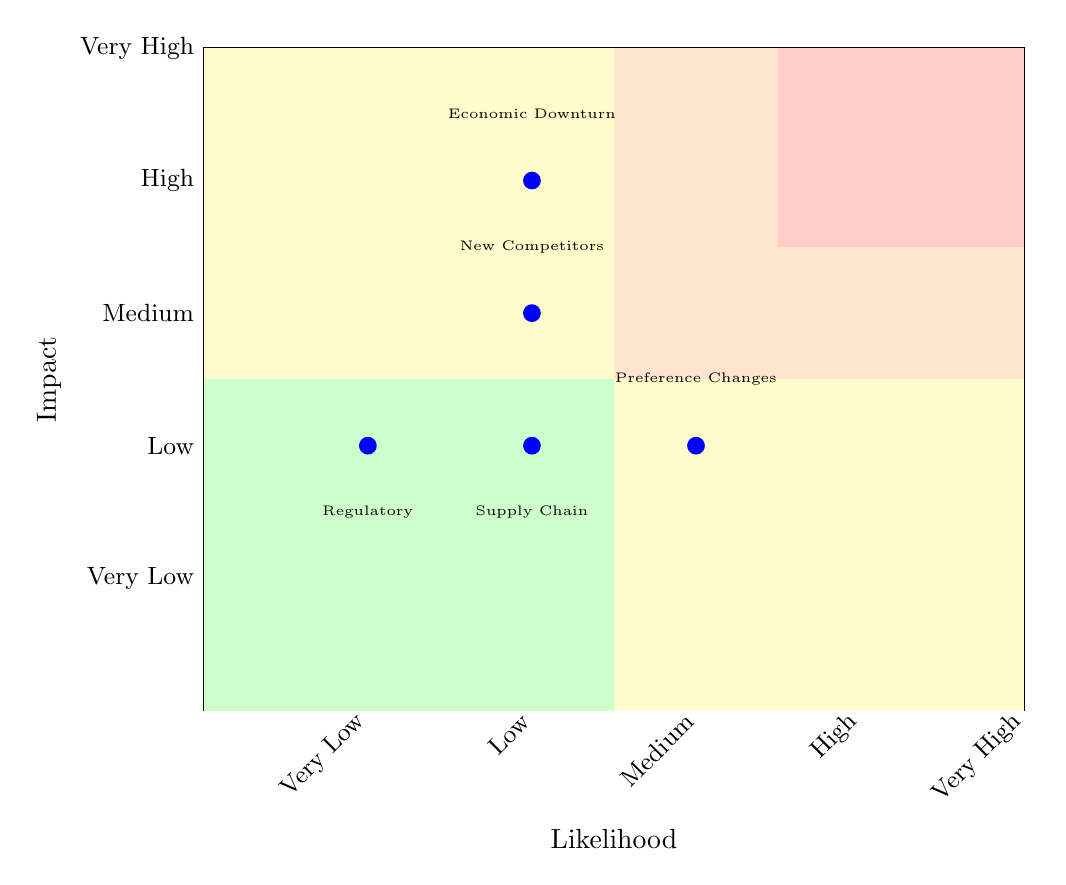
\begin{tikzpicture}
    \begin{axis}[
        xlabel={Likelihood},
        ylabel={Impact},
        xmin=0, xmax=5,
        ymin=0, ymax=5,
        grid=major,
        width=12cm,
        height=10cm,
        xtick={1,2,3,4,5},
        ytick={1,2,3,4,5},
        xticklabels={Very Low, Low, Medium, High, Very High},
        yticklabels={Very Low, Low, Medium, High, Very High},
        x tick label style={rotate=45, anchor=east, font=\small},
        y tick label style={font=\small}
    ]
    
    % Color zones
    \fill[green!20] (0,0) rectangle (2.5,2.5);
    \fill[yellow!20] (2.5,0) rectangle (5,2.5);
    \fill[yellow!20] (0,2.5) rectangle (2.5,5);
    \fill[orange!20] (2.5,2.5) rectangle (5,5);
    \fill[red!20] (3.5,3.5) rectangle (5,5);
    
    % Plot risks
    \addplot[only marks, mark=*, mark size=3pt, color=blue] 
        coordinates {(2,3)};
    \node at (axis cs:2,3.5) [font=\tiny] {New Competitors};
    
    \addplot[only marks, mark=*, mark size=3pt, color=blue] 
        coordinates {(2,4)};
    \node at (axis cs:2,4.5) [font=\tiny] {Economic Downturn};
    
    \addplot[only marks, mark=*, mark size=3pt, color=blue] 
        coordinates {(3,2)};
    \node at (axis cs:3,2.5) [font=\tiny] {Preference Changes};
    
    \addplot[only marks, mark=*, mark size=3pt, color=blue] 
        coordinates {(2,2)};
    \node at (axis cs:2,1.5) [font=\tiny] {Supply Chain};
    
    \addplot[only marks, mark=*, mark size=3pt, color=blue] 
        coordinates {(1,2)};
    \node at (axis cs:1,1.5) [font=\tiny] {Regulatory};
    
    \end{axis}
\end{tikzpicture}

\vspace{0.5em}
Most risks fall in low-to-medium zones with manageable mitigation strategies.
\end{center}

\vspace{2em}

% Business Success Factors Summary
\begin{center}
\textbf{Campus Glam Hub Success Framework}
\vspace{0.5em}

\begin{tikzpicture}[scale=0.9, transform shape]
    % Central circle
    \node[circle, draw=primarycolor, very thick, fill=primarycolor!20, minimum size=3cm, align=center, font=\bfseries] at (0,0) {Campus\\Glam Hub\\SUCCESS};
    
    % Surrounding factors
    \node[rectangle, draw, fill=secondarycolor!30, rounded corners, text width=2.5cm, align=center, drop shadow] at (0,4) {\textbf{Prime Location}\\On-campus\\convenience};
    
    \node[rectangle, draw, fill=secondarycolor!30, rounded corners, text width=2.5cm, align=center, drop shadow] at (3.5,2.5) {\textbf{Affordable Pricing}\\Student-friendly\\rates};
    
    \node[rectangle, draw, fill=secondarycolor!30, rounded corners, text width=2.5cm, align=center, drop shadow] at (3.5,-2.5) {\textbf{Quality Service}\\Professional\\standards};
    
    \node[rectangle, draw, fill=secondarycolor!30, rounded corners, text width=2.5cm, align=center, drop shadow] at (0,-4) {\textbf{Strong Marketing}\\Social media\\engagement};
    
    \node[rectangle, draw, fill=secondarycolor!30, rounded corners, text width=2.5cm, align=center, drop shadow] at (-3.5,-2.5) {\textbf{Customer Focus}\\Personalized\\care};
    
    \node[rectangle, draw, fill=secondarycolor!30, rounded corners, text width=2.5cm, align=center, drop shadow] at (-3.5,2.5) {\textbf{Skilled Team}\\Trained\\professionals};
    
    % Connecting lines
    \foreach \angle in {0,60,120,180,240,300} {
        \draw[thick, primarycolor] (0,0) -- (\angle:2);
    }
    
\end{tikzpicture}
\end{center}

